%\newcommand*{\SCRIPT}{}
\newcommand*{\BEAMER}{}

\ifdefined\SCRIPT
	\documentclass{article}
	\usepackage[a4paper, left=2.5cm, right=2cm, top=5.5cm, bottom=2.5cm]{geometry}
	\usepackage[noxcolor]{beamerarticle}
	\usepackage[ngerman]{babel}
	\usepackage[utf8]{inputenc}
	\usepackage{amsmath}
	\usepackage{amsthm}
	\usepackage{graphicx}
	\usepackage{pgfplots}
	\usepackage{tcolorbox}
	\usepackage{siunitx}
	\sisetup{locale = DE,
	per-mode=fraction}
	\usetikzlibrary{arrows,patterns}
	\usepackage{biblatex}
	\usepackage{xltabular}
	\usepackage{scrlayer-scrpage}
	\pagestyle{scrheadings}
	\clearpairofpagestyles
	\ofoot{Seite \pagemark}
	\newcolumntype{C}[1]{>{\centering\arraybackslash}p{#1}}
	\DeclareNewLayer[%
	  background,% Hintergrundebene
	  width=\textwidth,% Größe und Position des Textbereichs
	  hoffset=2.5cm,
	  voffset=2.5cm,
	  align=tl,
	  contents={%
	  \sffamily
	    \setlength{\fboxsep}{2mm}% Abstand Box Text
	    \setlength{\fboxrule}{.5mm}% Dicke Linie
	    % vertikale Position korrigieren    
	    \vskip-\fboxsep\vskip-\fboxrule\vskip-\baselineskip
	    % horizontale Position korrigieren
	    \hspace{-\fboxsep}\hspace{-\fboxrule}%
	    \begin{tabularx}{\textwidth}{|>{\bfseries\Large}C{7cm}|X|X|}                                                       
	\hline
	\vspace{0em}
\includegraphics[scale=0.3]{logo2.png} & Name: & Datum: \\
	\hline
	
	\end{tabularx}
	    %\makebox[\layerwidth][l]{%
	    %  \fbox{\rule{0pt}{\layerheight}\rule{\layerwidth}{0pt}}% Rahmen
	    %}%
	  }
	]{frame}
	\AddLayersToPageStyle{@everystyle@}{frame}
\fi

\ifdefined\BEAMER
	\documentclass{beamer}
	\usepackage[ngerman]{babel}
	\usepackage[utf8]{inputenc}
	\usepackage{amsmath}
	\usepackage{amsthm}
	\usepackage{siunitx}
	\usepackage{graphicx}
	\usepackage{pgfplots}
	\usepackage{svg}
	\sisetup{locale = DE,
	per-mode=fraction}
	% Lade Beamer Stile
	\usepackage{beamerthemesplit}
	\usepackage{tcolorbox}
	\usetheme{Rochester}
	\usecolortheme{crane}
	\usetikzlibrary{arrows,patterns}
\fi

\title{1. Unterrichtseinheit zur Wärmelehre}
\subtitle{Einführung in die Wärmelehre}
\author{Heiko Schröter}
\date{\today}

\setbeamertemplate{enumerate item}{\alph{enumi})}

\begin{document}

\frame{\titlepage}

\frame
{
  \frametitle{Wärmelehre}
  Die Wärmelehre beschäftigt sich mit dem Wärmezustand von Körpern, den Wärmemengen und den Eigenschafts- und Zustandsänderungen von Stoffen bei unterschiedlichen Wärmezuständen.
    \begin{figure}
	  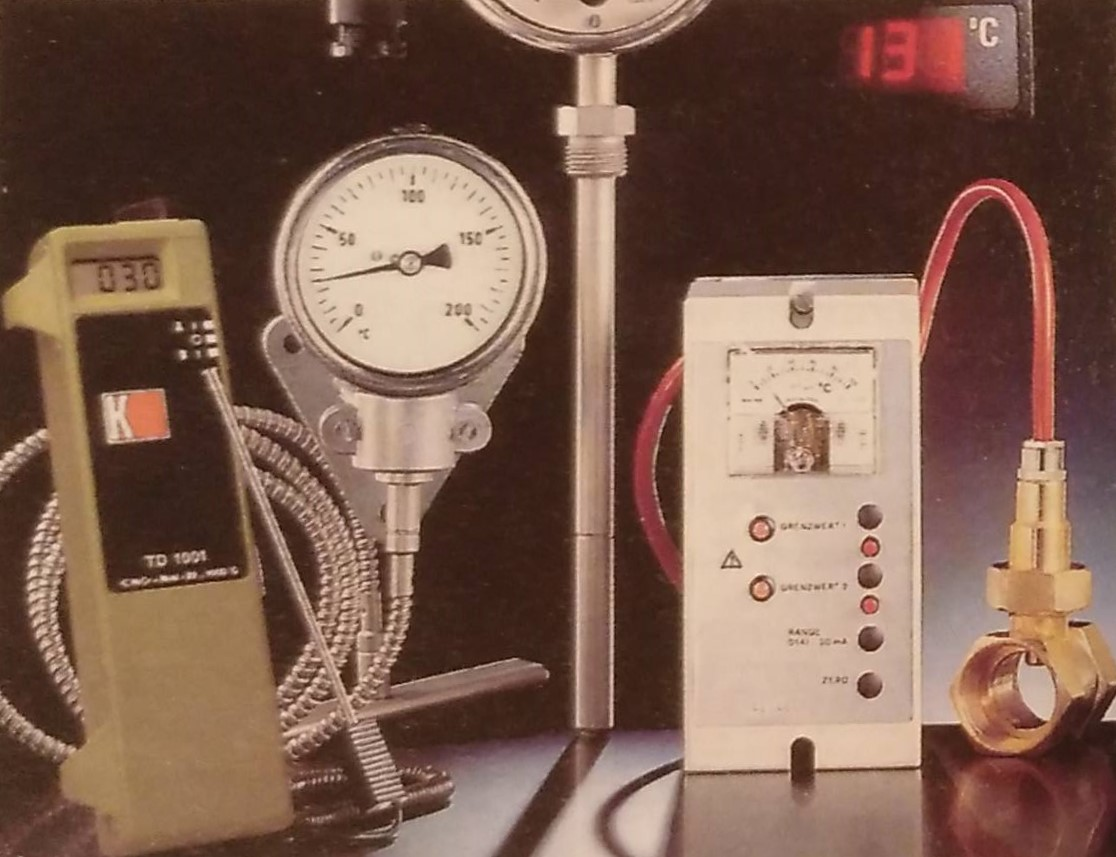
\includegraphics[width=0.5\textwidth]{Wärmelehre.jpg}
	  \vspace{-3mm}
	  \caption{Temperaturmessgeräte der Technik}
   \end{figure}  
}

\frame
{
  \frametitle{Ziele für die heutige Unterrichtseinheit}
  \textbf{Einführung in die Wärmelehre}
  \begin{itemize}
	\item Beschreibung der Temperatur als Zustandsgröße
	\item Herausarbeiten der Temperaturskalen
	\item Welche Temperaturmessverfahren gibt es?
	\item Beschreibung der Wärme als Energieform
	\item Wie sieht die Temperaturkurve beim Erwärmen von Eis aus?
  \end{itemize}
}

\frame[allowframebreaks]
{
  \frametitle{Temperatur als Zustandsgröße}
  \begin{block}{}
  Das Temperaturempfinden ist subjektiv und deshalb zur Temperaturermittlung ungeeignet.
  \end{block}
   \begin{figure}
	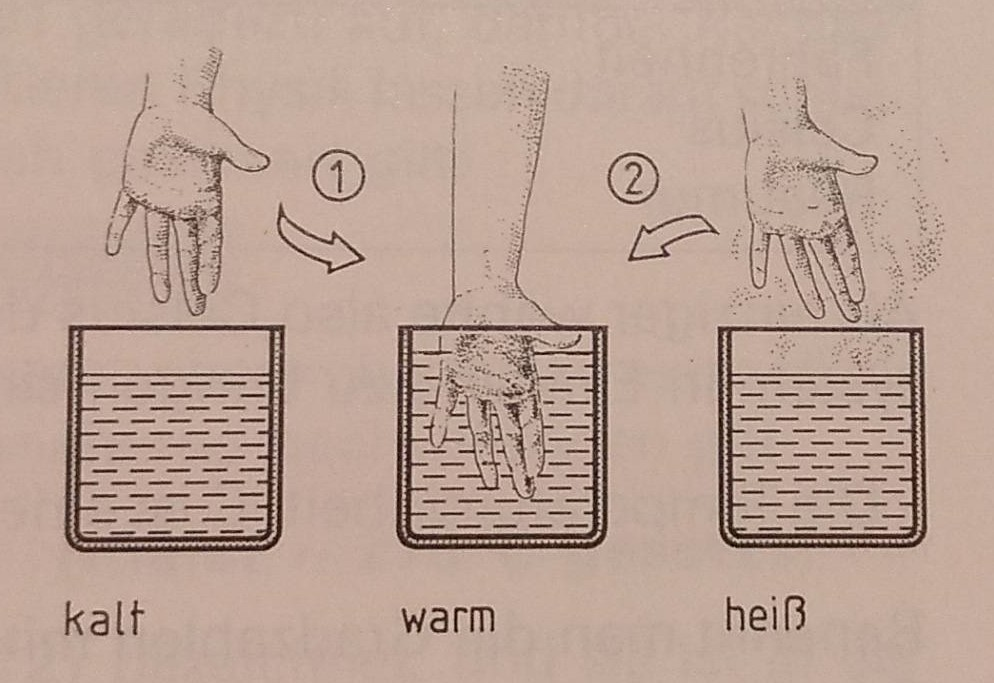
\includegraphics[width=0.5\textwidth]{Temperatur.jpg}
	\vspace{-3mm}
	\caption{subjektives Wärmeempfinden}
   \end{figure}
  \begin{block}{}
  Temperatur ist eine messbare Größe, eine Zustandsgröße und ist eine skalare (richtungsunabhängige) Größe.
  \end{block}
  \begin{itemize}
  \item Die SI-Basiseinheit der Temperatur ist das \textbf{Kelvin}\footnote[frame]{Lord William Kelvin, englischer Physiker (1824 bis 1907)} mit dem Kurzzeichen \textbf{K} und dem Formelzeichen $T$.\\
  \item Im Alltagsleben und in der Technik wird überwiegend die \textbf{Celsius-Temperaturskala}\footnote[frame]{Anders Celsius, schwedischer Physiker (1701 bis 1744)} verwendet, mit dem Formelzeichen $\vartheta$. 
  \end{itemize}
}

\frame[allowframebreaks]
{
  \frametitle{Temperaturskalen}
  \begin{tikzpicture}
    \begin{axis}[
	%axis x line=center,
	title=$\vartheta$ - t -Diagramm für Wasser,
	%xlabel=Zeit t,
	ylabel=Temperatur $\vartheta$,
	xmin=0, xmax=50,
	ymin=-20, ymax=150,
	xtick=\empty,
 	enlargelimits=false
]
	\addplot [color=red, thick, mark=no, domain=0:40] coordinates {
    (4, -10)
    (5, 0)
    (10, 0)
    (15, 50)
    (20, 100)
    (25, 100)
    (30, 100)
    (35, 140)
	};
	\draw[help lines, dashed] {(axis cs:0,0) -- (axis cs:50,0)
	(axis cs:0,100) -- (axis cs:50,100)};
	\node [fill=white] at (axis cs:40,0) {Eispunkt};
	\node [fill=white] at (axis cs:40,100) {Siedepunkt};
	\coordinate (A) at ({axis cs:0,0});
    \coordinate (B) at ({axis cs:0,100});
    \draw[<->, >=latex] (axis cs:25,0) -- node[midway, align=center, rotate=90]{Fundamental- \\ abstand} (axis cs:25,100);
\end{axis}
  \node[pin={above right:$\vartheta_{1}$}] at (A) {};
  \node[pin={above right:$\vartheta_{2}$}] at (B) {};
\end{tikzpicture}

  \begin{block}{Die Celsius-Skala}
  Wasser schmilzt bzw. erstarrt (gefriert), und Wasser siedet (verdampft) bzw. kondensiert (verflüssigt) in Abhängigkeit vom vorhandenen Luftdruck, bei einer bestimmten, d.h. festen Temperatur.
  \end{block}  
}

\frame
{
  \frametitle{Temperaturskalen}
  \begin{tikzpicture}
  \begin{scope}[scale=0.013]
    \fill [lightgray] (0,-100) -- (0,-200) -- (300,-200) -- (300,-100) -- cycle;
    \draw [->, >=latex, thick] (0,-273.15) -- (0,200) node [left] {$\vartheta$ in \si{\celsius}};
    \draw [->, >=latex, thick] (300,-273.15) -- (300,200) node [right] {$T$ in \si{\kelvin}};
    \draw (-10,-273.15) node [left] {$\vartheta_0=\SI{-273.15}{\celsius}$} -- (310,-273.15) node [right] {$T_0=\SI{0}{\kelvin}$};
    \draw (-10,-200) node [left] {$\vartheta_1$} -- (310,-200) node [right] {$T_1$};
    \draw (-10,-100) node [left] {$\vartheta_2$} -- (310,-100) node [right] {$T_2$};
    \draw (-10,0) node [left] {\SI{0}{\celsius}} -- (310,0) node [right] {\SI{273.15}{\kelvin}};
    \draw (-10,100) node [left] {\SI{100}{\celsius}} -- (310,100) node [right] {\SI{373.15}{\kelvin}};
    \draw [<->, >=latex] (90,-100) -- node [midway, right] {$\Delta\vartheta=\Delta T$} (90,-200);
  \end{scope}
  \end{tikzpicture}
}

\frame{
  \frametitle{Welche Temperaturmessverfahren gibt es?}
  \begin{block}{Die Temperaturmessverfahren sind immer indirekte Messverfahren.}
  Körperfarbe, Körperform, Abmessungen der Körper, Elektrischer Widerstand, Kontaktspannung
  \end{block}

\begin{itemize}
  \item Flüssigkeitsthermometer
  \item Bimetallthermometer
  \item Elektrisches Widerstandsthermometer
  \item Das Thermoelement
  \item Pyrometer
  \item Segerkegel
  \item Thermochromfarben
  \item Thermographie
\end{itemize}
}

\frame{
  \frametitle{Welche Temperaturmessverfahren gibt es?}
  \begin{exampleblock}{Flüssigkeitsthermometer}
\begin{center}
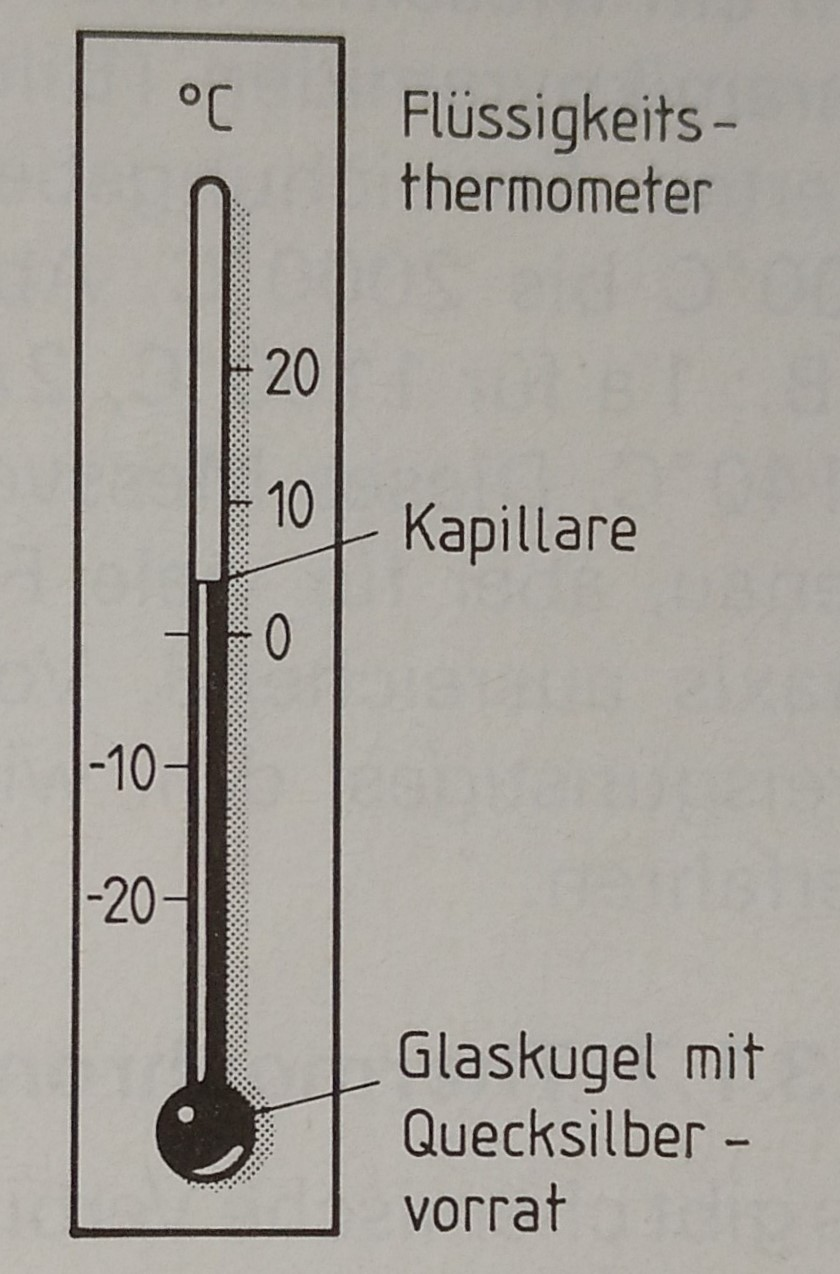
\includegraphics[scale=0.1]{Flüssigkeitsthermometer.jpg} 
\end{center}
  \end{exampleblock}
Veränderung des Volumens
}

\frame{
  \frametitle{Welche Temperaturmessverfahren gibt es?}
  \begin{exampleblock}{Bimetallthermometer}
\begin{center}
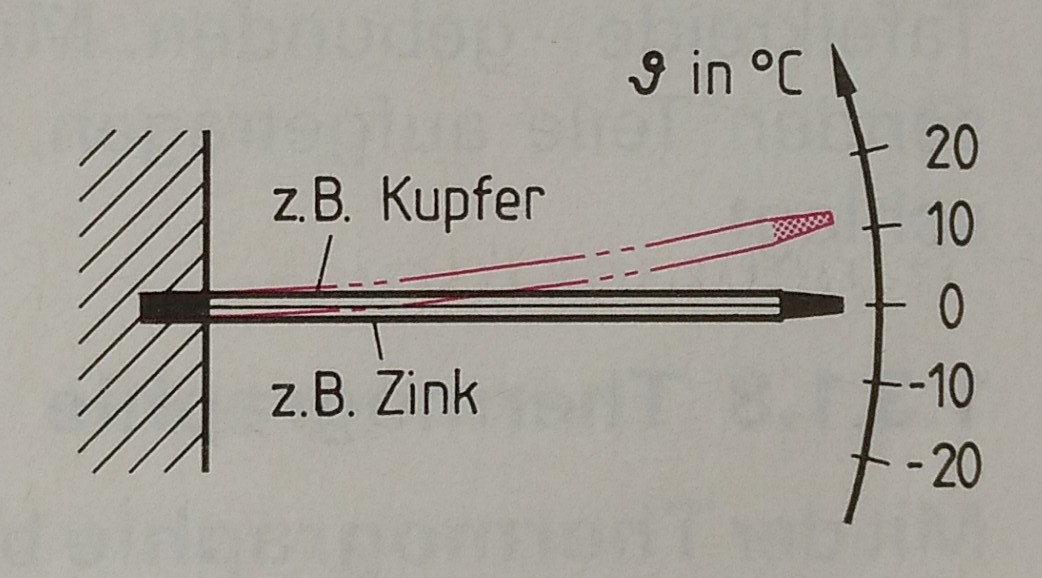
\includegraphics[scale=0.2]{Bimetallthermometer.jpg} 
\end{center}
  \end{exampleblock}
unterschiedlicher Längenausdehnungskoeffizient
}

\frame{
  \frametitle{Welche Temperaturmessverfahren gibt es?}
  \begin{exampleblock}{Elektrisches Widerstandsthermometer}
\begin{center}
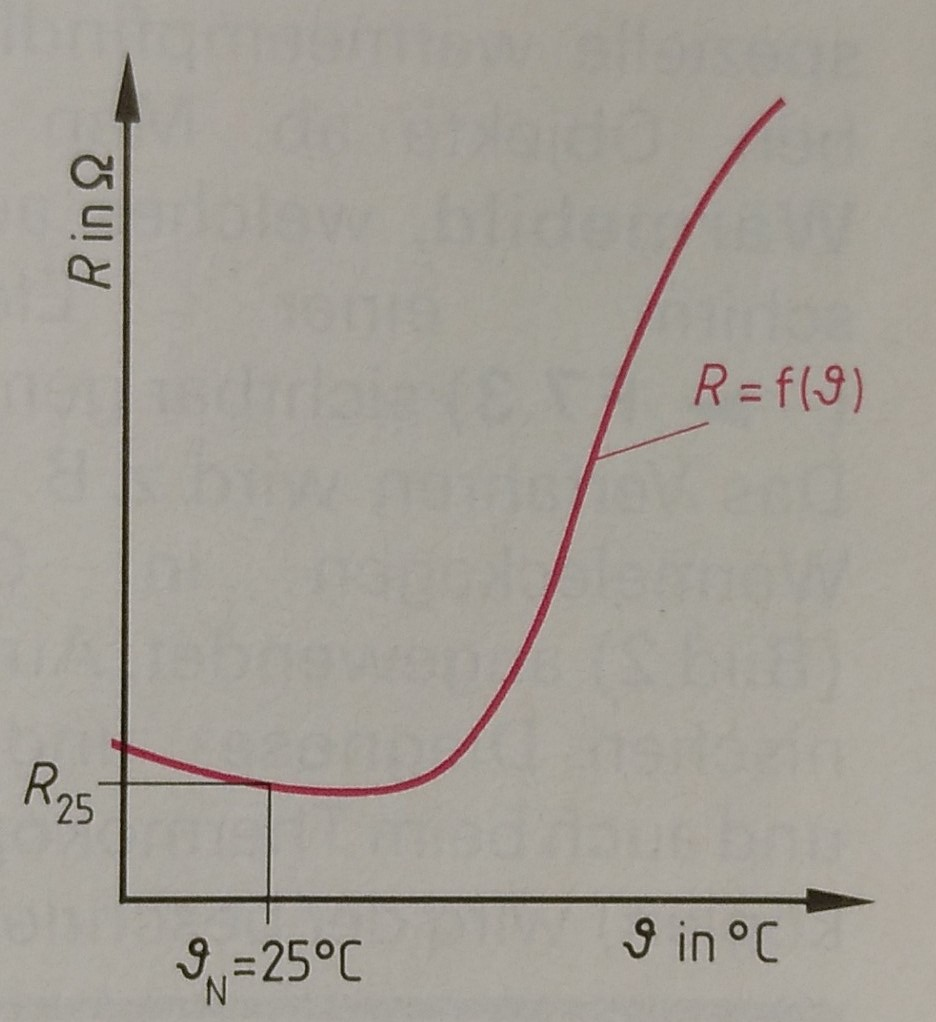
\includegraphics[scale=0.12]{Widerstandsthermometer} 
\end{center}
  \end{exampleblock}
Änderung des elektrischen Widerstands
}

\frame{
  \frametitle{Welche Temperaturmessverfahren gibt es?}
  \begin{exampleblock}{Thermoelement}
\begin{center}
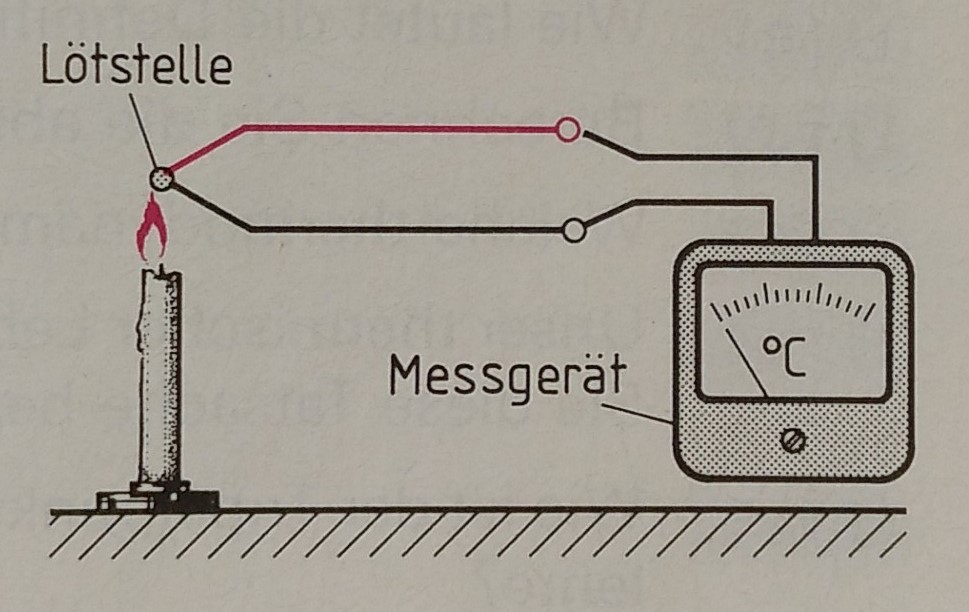
\includegraphics[scale=0.15]{Thermoelement} 
\end{center}
  \end{exampleblock}
Änderung der Thermospannung
}

\frame{
  \frametitle{Welche Temperaturmessverfahren gibt es?}
  \begin{exampleblock}{Pyrometer}
\begin{center}
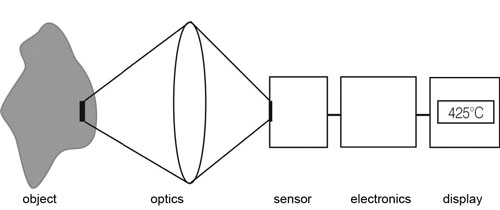
\includegraphics[scale=0.4]{Pyrometer} 
\end{center}
  \end{exampleblock}
Änderung der Wärmestrahlung (IR-Strahlung)
}

\frame{
  \frametitle{Welche Temperaturmessverfahren gibt es?}
  \begin{exampleblock}{Segerkegel}
\begin{center}
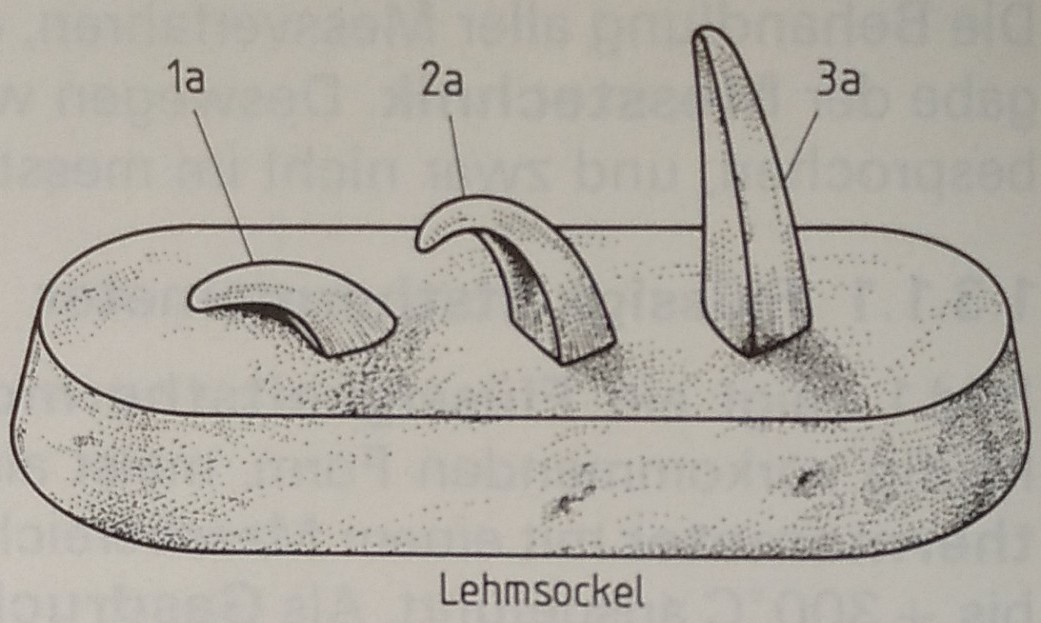
\includegraphics[scale=0.2]{Segerkegel} 
\end{center}
  \end{exampleblock}
Veränderung der Form
}

\frame{
  \frametitle{Welche Temperaturmessverfahren gibt es?}
  \begin{exampleblock}{Thermochromfarben}
  \begin{figure}
	\begin{center}
		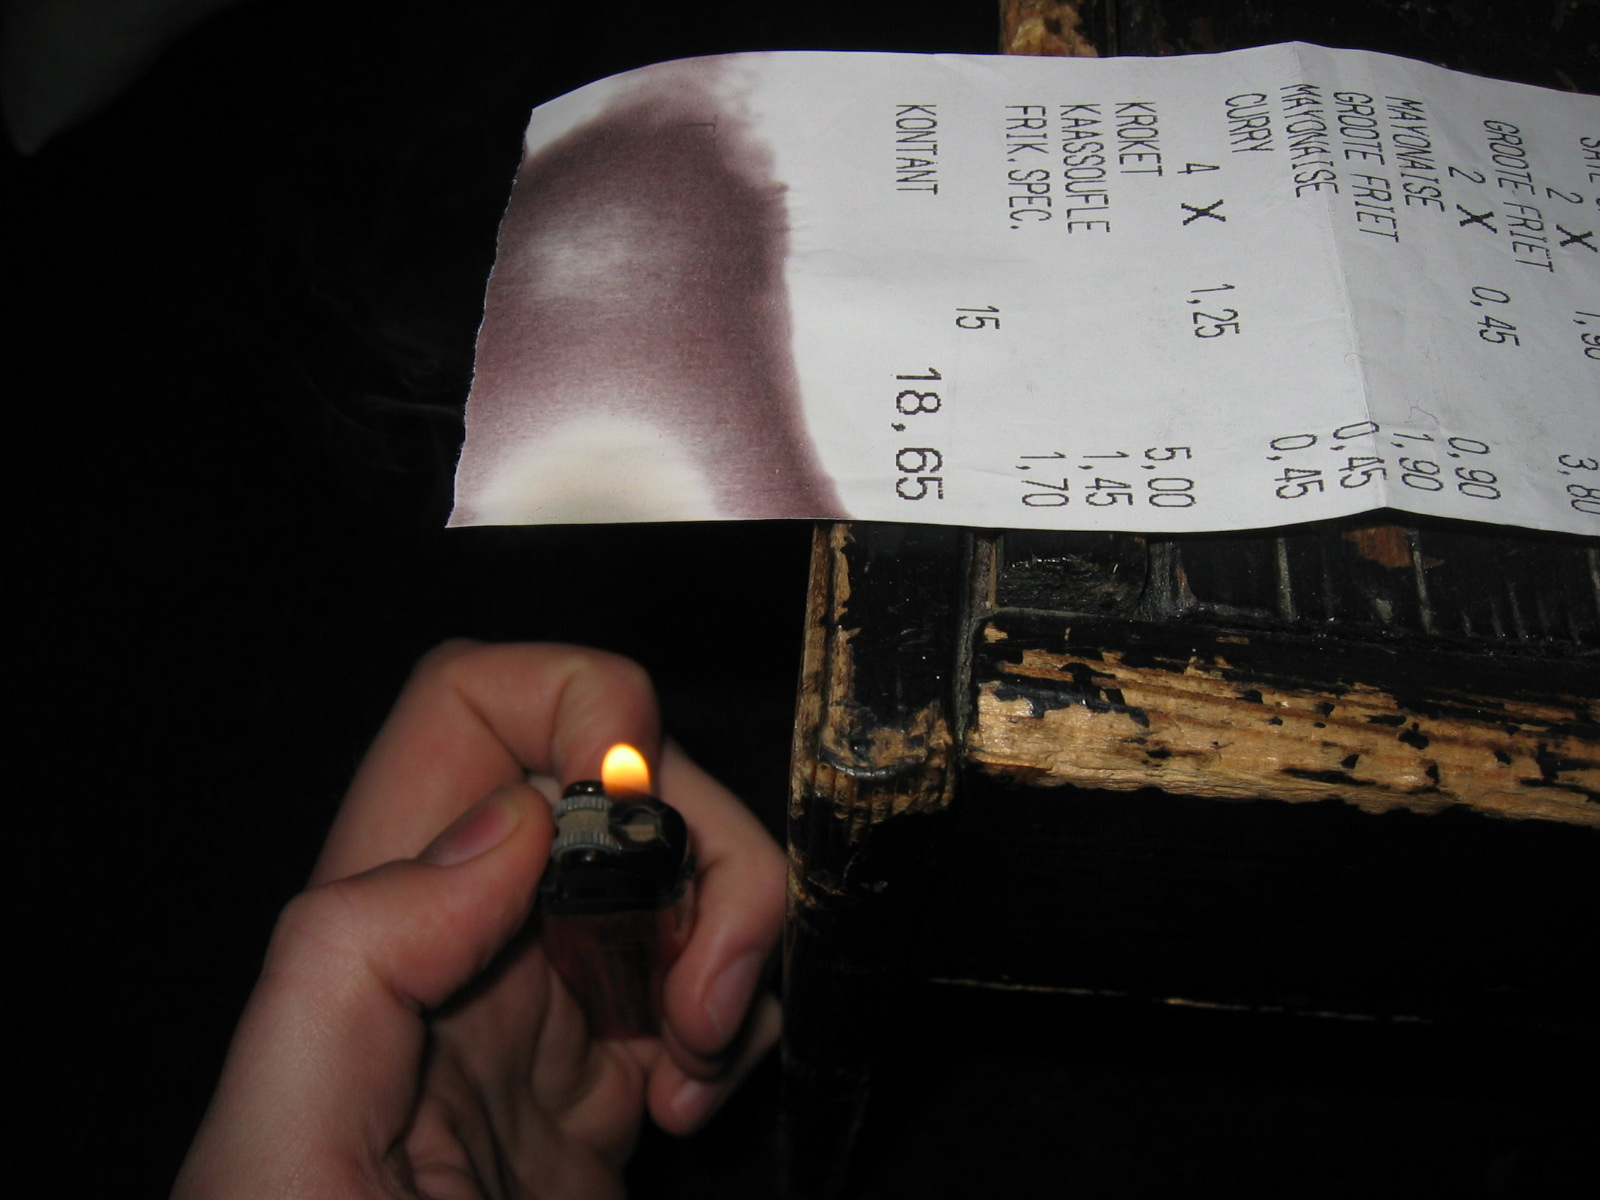
\includegraphics[scale=0.2]{Thermal_paper} 
	\end{center}
	\caption{Von IIVQ - Tijmen Stam - Eigenes Werk, CC BY-SA 3.0, https://commons.wikimedia.org/w/index.php?curid=804449}
  \end{figure}
  \end{exampleblock}
Veränderung der Farbe
}

\frame{
  \frametitle{Welche Temperaturmessverfahren gibt es?}
  \begin{exampleblock}{Thermographie}
\begin{center}
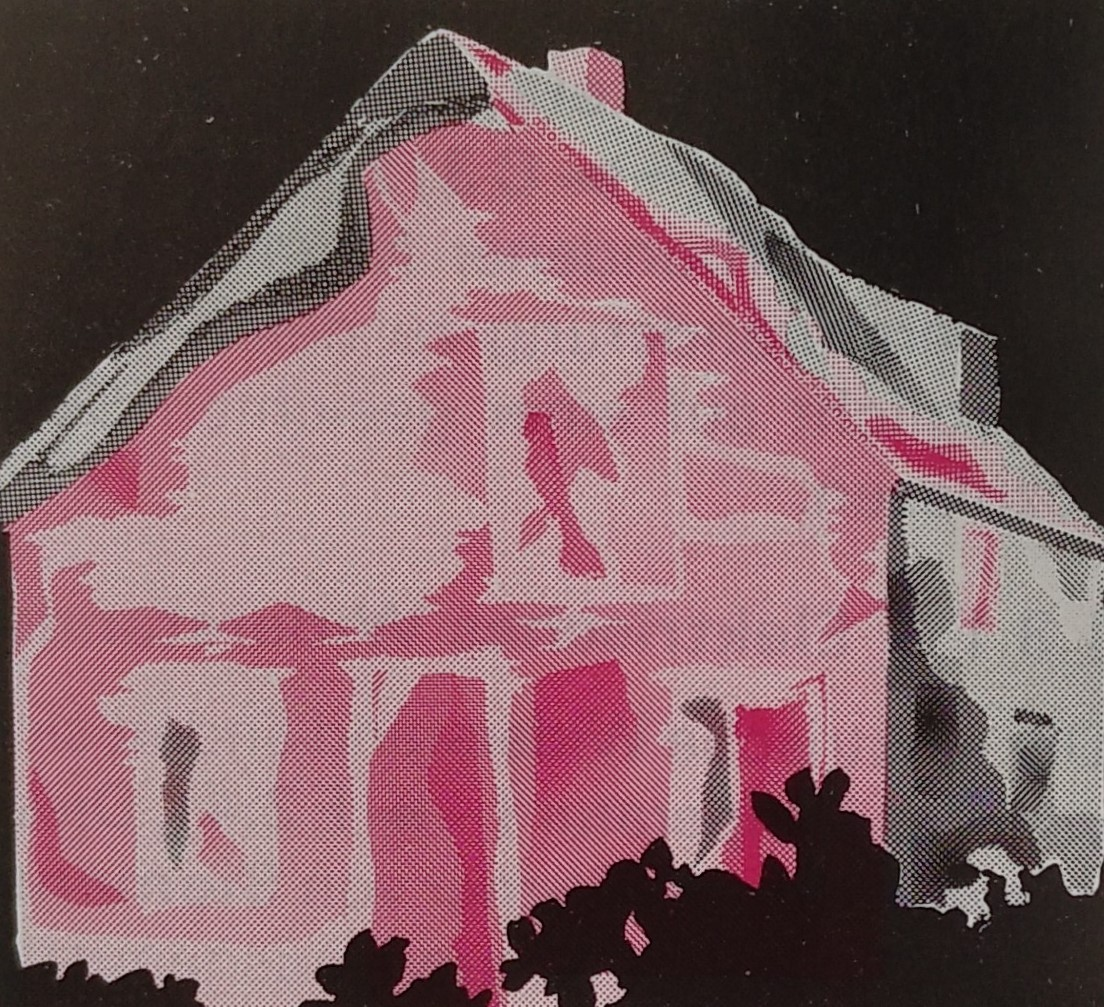
\includegraphics[scale=0.1]{Thermographie} 
\end{center}
  \end{exampleblock}
Änderung der Wärmestrahlung (IR-Strahlung)
}

\frame[allowframebreaks]
{
  \frametitle{Beschreibung der Wärme als Energieform}
  \begin{block}{Energie kann in verschiedenen Arten auftreten, und ist meist von einer Art in eine andere Art umwandelbar.}
  \begin{itemize}
  \item Mechan. Energie
  \item Kernenergie
  \item Chemische Energie
  \item Elektrische Energie
  \item Druckenergie
  \item Wärmeenergie u.a.
  \end{itemize}
  \end{block}
\begin{center}
Simulation von Temperaturänderungen mittels Algoodo
  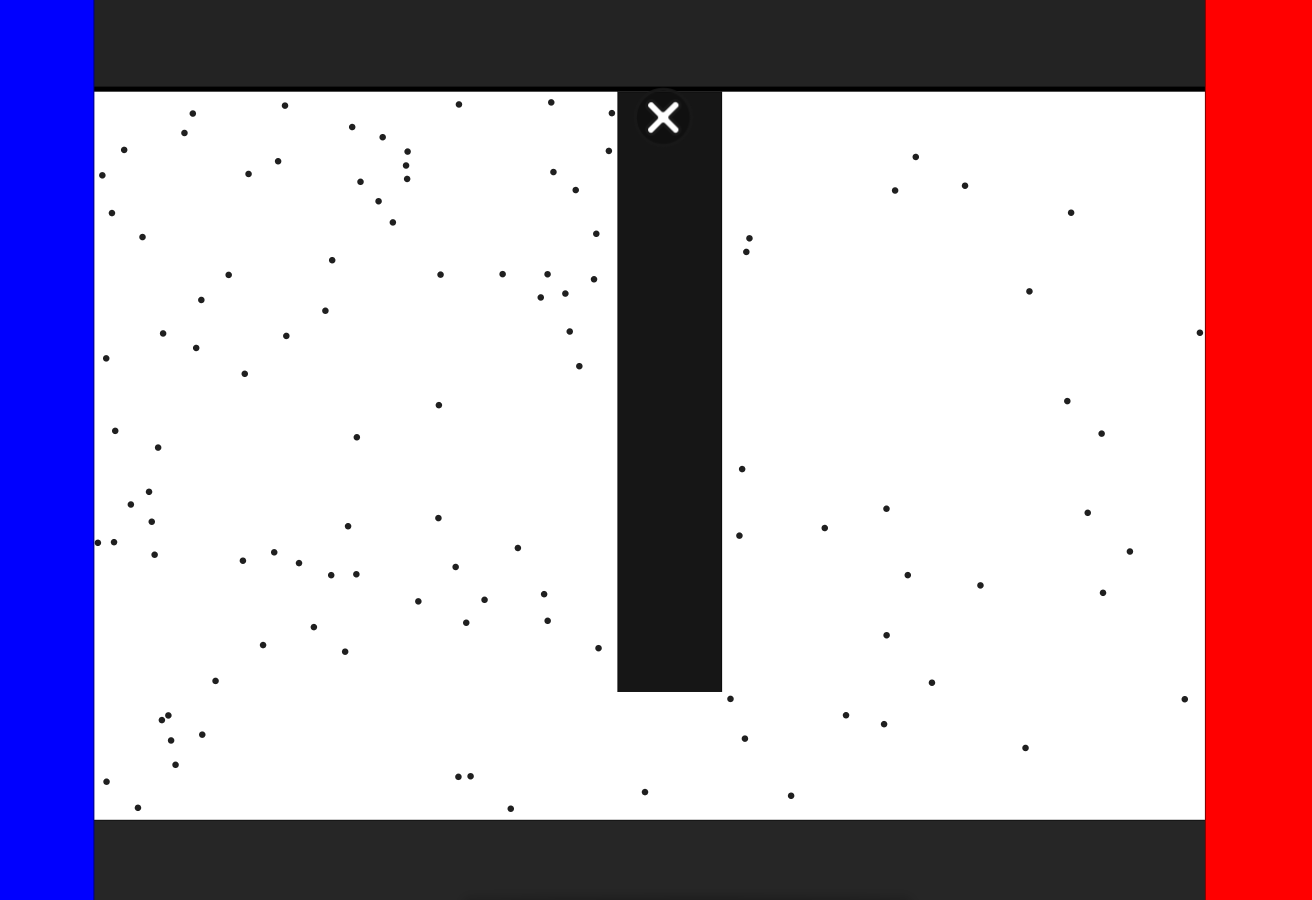
\includegraphics[scale=0.05]{Temperatur.png} 
\end{center}
  \newpage
  \begin{block}{}
Die Wärme ist eine Energieform. Man bezeichnet sie als Wärmeenergie.
  \end{block}
	\begin{itemize}
	  \item Die SI-Einheit der Wärmeenergie ist die Energieeinheit \\\textbf{Joule}\footnote[frame]{James Prescot Joule, englischer Physiker (1818 bis 1889)} mit dem Kurzzeichen $\si{\joule}$ und dem Formelzeichen $Q$.
	  \item Im Alltagsleben und in der Technik werden häufig die größeren Einheiten Kilojoule ($\si{\kilo\joule}$) und Megajoule ($\si{\mega\joule}$) verwendet.
	\begin{tcolorbox}	  
	  $\SI{1}{\joule} = \SI{1}{\newton\meter} = \SI{1}{\watt\second}$
	\end{tcolorbox}
	\newpage
	  \item Die früher gebräuchliche Einheit der Wärmeenergie war die \textbf{Kilokalorie}.
	\end{itemize}	
	\begin{tcolorbox}	  
	  $1 \text{kcal} \approx \SI{4.19}{\kilo\joule}$
	\end{tcolorbox}
  \begin{block}{Der Mechanismus der Wärmespeicherung}
  Bei Zuführung von Wärmeenergie erhöht sich die Bewegungsenergie der Elementarbausteine und umgekehrt nimmt diese bei Wärmeabfuhr ab.
  \end{block}
  \newpage
\begin{center}
Simulation Zuführung von Wärmeenergie\\
  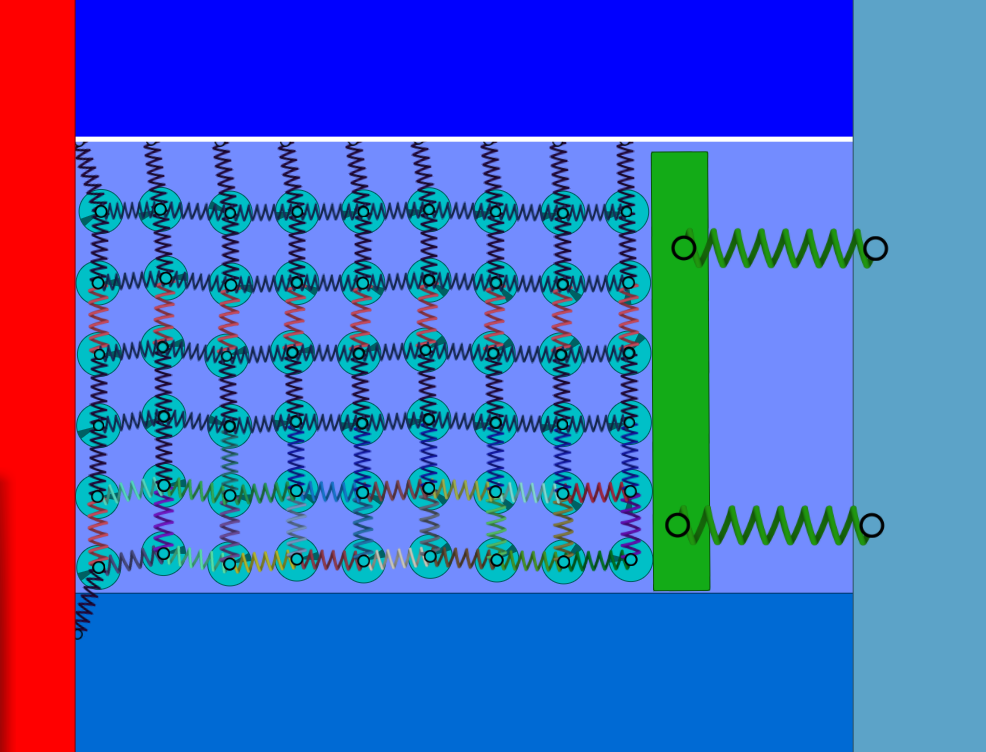
\includegraphics[scale=0.3]{Wärme.png} 
\end{center}  
}

\frame[allowframebreaks]
{
  \frametitle{Temperaturverlauf beim Erwärmen von Eis}
  \begin{tikzpicture}
    \begin{axis}[
	%axis x line=center,
	title=$\vartheta$ - t -Diagramm für Wasser,
	%xlabel=Zeit t,
	ylabel=Temperatur $\vartheta$,
	xmin=0, xmax=50,
	ymin=-20, ymax=150,
	xtick=\empty,
 	enlargelimits=false
]
	\addplot [color=red, thick, mark=no, domain=0:40] coordinates {
    (4, -10)
    (5, 0)
    (10, 0)
    (15, 50)
    (20, 100)
    (25, 100)
    (30, 100)
    (35, 140)
	};
	\draw[help lines, dashed] {(axis cs:0,0) -- (axis cs:50,0)
	(axis cs:0,100) -- (axis cs:50,100)};
	\node [fill=white] at (axis cs:40,0) {Eispunkt};
	\node [fill=white] at (axis cs:40,100) {Siedepunkt};
	% \coordinate (A) at ({axis cs:0,0});
    % \coordinate (B) at ({axis cs:0,100});
    \draw[<->, >=latex] (axis cs:25,0) -- node[midway, align=center, rotate=90]{Fundamental- \\ abstand} (axis cs:25,100);
    \draw[<-, >=latex, blue] (axis cs:12,20) -- (axis cs:17,20) node[right]{$Q_3$};
	\draw[<-, >=latex, blue] (axis cs:4,-9) -- (axis cs:9,-9) node[right]{$Q_1$};
	\draw[<-, >=latex, blue] (axis cs:32.5,120) -- (axis cs:37.5,120) node[right]{$Q_5$};
	\draw[<-, >=latex, blue] (axis cs:7.5,0) -- (axis cs:5,12) node[left]{$Q_2$};
	\draw[<-, >=latex, blue] (axis cs:25,100) -- (axis cs:22.5,112) node[left]{$Q_4$};
\end{axis}
   % \node[pin={above right:$\vartheta_{1}$}] at (A) {};
   % \node[pin={above right:$\vartheta_{2}$}] at (B) {};
 \end{tikzpicture}
\begin{tabular}{ll}
$Q_1\rightarrow$ & Temperaturerhöhung bis \SI{0}{\celsius} \\ 
$Q_2\rightarrow$ & Schmelzen des Eises bei \SI{0}{\celsius} \\ 
$Q_3\rightarrow$ & Temperaturerhöhung von \SI{0}{\celsius} bis \SI{100}{\celsius} \\ 
$Q_4\rightarrow$ & Verdampfen des Wassers bei \SI{100}{\celsius} \\ 
$Q_5\rightarrow$ & Temperaturerhöhung des Dampfes über \SI{100}{\celsius} \\ 
\end{tabular} 
  \begin{block}{Sensible und latente Wärmeenergie}
\begin{tabular}{ll}
sensible Wärme & Die zu- oder abgeführte Energie ändert die\\
& Körpertemperatur. \\ 
\hline 
latente Wärme & Die zu- oder abgeführte Energie ändert den\\
& Aggregatzustand oder die Gitterstruktur des\\
& Körpers bei konstanter Temperatur. \\ 
\end{tabular} 
  \end{block}
}

\end{document}
